\chapter{What Governs the Loss: Order Error and What the Known Bound
Does Not
Say}

Chapter 4 showed that on average-case inputs the loss of a
degree-prediction algorithm is small. This chapter asks what
\emph{governs} that loss. MinPredictedDegree matches by ascending
predicted degree, so it depends on the predictor \(\mu\) \emph{only
through the order it induces} on the resources: two predictors inducing
the same order produce identical matchings, and a monotone rescaling of
\(\mu\) changes nothing. The right question is therefore not ``how large
is the error'' but ``which \emph{order} error governs the loss, and how
tightly.'' Answering it requires care, because the qualitative fact that
order, not magnitude, matters is already a theorem, and we are explicit
about what is prior and what is ours.

\section{What is already known (ACI)}

Aamand, Chen and Indyk \autocite[Appendix D]{aci2022mpd} prove that on
the CLV-B model, MinPredictedDegree's matching loss relative to the true
expected degrees is at most \(n-\mathrm{LIS}(w[\mu])\). Here \(w\) is
the vector of true expected degrees (written \(w\) rather than \(p\) to
keep it distinct from the type distribution \(p\) of §3.1), \(w[\mu]\)
is that vector listed in the order \(\mu\) induces, and \(\mathrm{LIS}\)
is the length of its longest non-decreasing subsequence: a pure
\emph{order} quantity. In particular a monotone (order-preserving)
predictor leaves \(w[\mu]\) already sorted, so \(n-\mathrm{LIS}=0\) and
the loss is zero. Thus \emph{order-dependence} and \emph{the zero-effect
of a monotone bias} are ACI's results, not ours; our systematic-bias
error model (a monotone rescale) has Kendall-\(\tau\equiv0\) by
construction and, consistently, leaves MPD's ratio exactly unchanged
across the benchmark (Chapter 4): an empirical confirmation of ACI's
statement, not a new finding.

\section{Our characterization}

We sweep the four structured error models across strength and record,
per model and level on the same instances, three quantities: the actual
MPD matching loss, ACI's \(n-\mathrm{LIS}\), and the normalized
Kendall-\(\tau\) order error, reported on \([0,1]\), where \(0\) means
the predicted order is exactly right and \(1\) that it is exactly
reversed (\textbf{Figure 5.1}; \(n=1000\), Zipf exponent \(1.0\), 40
trials).

\begin{figure}
\centering
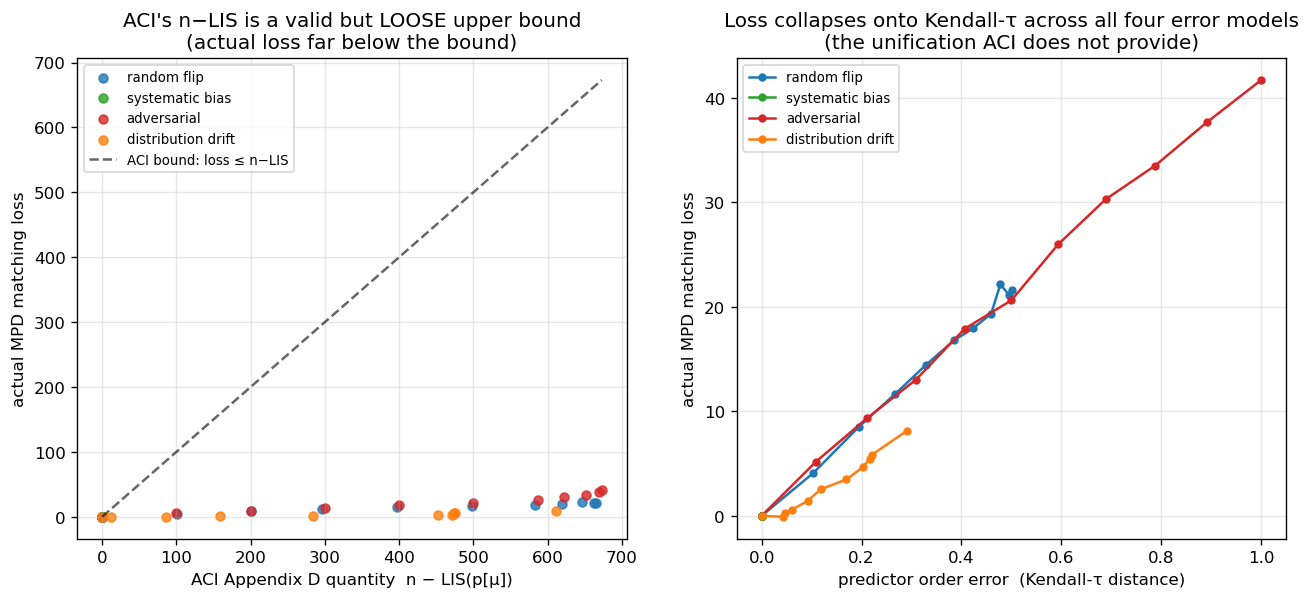
\includegraphics[width=1\linewidth,height=\textheight,keepaspectratio,alt={Order error governs the loss: the realized loss lies far below ACI's n-\textbackslash mathrm\{LIS\} bound (a) and collapses onto Kendall-\textbackslash tau across all four error models (b).}]{../../results/order_vs_theory.png}
\caption{Order error governs the loss: the realized loss lies far below
ACI's \(n-\mathrm{LIS}\) bound (a) and collapses onto Kendall-\(\tau\)
across all four error models (b).}
\end{figure}

\textbf{(i) ACI's \(n-\mathrm{LIS}\) bound is correct but very loose.}
The realized loss lies far below the bound at every point. Taking the
ratio of the bound to the realized loss at each model's strongest
corruption level, it is loose by roughly \(16\times\) (adversarial) to
\(75\times\) (distribution-drift); all points hug the axis in Figure
5.1(a).

\textbf{(ii) \(n-\mathrm{LIS}\) saturates and cannot distinguish error
structures.} For every non-trivial error it is pinned near its maximum
(\(\approx610\)--\(673\) out of a possible \(n=1000\), against realized
losses of \(8\) to \(42\)), even though the true losses differ by a
factor of five across models (\(8.1\) drift, \(21.6\) random-flip,
\(41.7\) adversarial). As a bound that is almost always \(\approx n\),
it carries little information about which prediction is more harmful.

\textbf{(iii) Kendall-\(\tau\) is the governing order measure, and the
models collapse onto it.} Plotted against Kendall-\(\tau\) (Figure
5.1(b)), the four models fall on one increasing curve : loss rises with
\(\tau\) (\(0.29\to0.50\to1.0\) for drift, random-flip, adversarial,
tracking \(8.1\to21.6\to41.7\)), with systematic bias pinned at
\(\tau=0\), zero loss. The collapse is not only visual: pooling all four
models and all error levels (44 points), the rank correlation between
Kendall-\(\tau\) and the realized loss is Spearman \(\rho=0.979\)
(Pearson \(r=0.992\)), and within each non-degenerate model it is
\(0.97\) or above. The quantity that \emph{predicts} the loss and
unifies the error structures is the Kendall-\(\tau\) order distance,
which the saturated \(n-\mathrm{LIS}\) cannot resolve.

\section{Chapter summary}

What this chapter adds, order-dependence itself being ACI's result
(§5.1), is a precise empirical characterization of how much the known
bound actually says: ACI's \(n-\mathrm{LIS}\) bound is loose by one to
nearly two orders of magnitude and saturates, whereas Kendall-\(\tau\)
predicts the realized loss and unifies the four error structures. This
both sharpens the theory's practical content and justifies the single
order-error axis used when the predictor is stressed on real data. It is
also why Chapter 7 can explain a cheap historical predictor's success by
its order fidelity alone, and why Chapter 8 tried, and failed, to train
a predictor for order directly.
